% preamble-exam-zh.tex — 极简讲解页共享 preamble
% 目标：复刻「题目独立、提示轻框、路线箭头、主体双栏、答案轻收束」的讲义风格。

\documentclass{exam-zh}

% ---------- 基础配置 ----------
\examsetup{
  page/size = a4paper,
  page/show-head = false,
  page/show-foot = false,
  sealline/show = false,
  font = none,
  math-font = none,
}

% ---------- 包 ----------
\usepackage{geometry}
\geometry{top=10mm,bottom=14mm,left=12mm,right=10mm}
\AtBeginDocument{\newgeometry{top=10mm,bottom=14mm,left=12mm,right=10mm}}

\usepackage{xcolor}
\usepackage{needspace}
\usepackage{enumitem}
\usepackage{array}
\usepackage{tabularx}
\usepackage{tcolorbox}
\tcbuselibrary{skins,breakable}
\usepackage{paracol}
\usepackage{graphicx}
\usepackage{tikz}
\usetikzlibrary{calc,intersections,angles,quotes,arrows.meta,decorations.markings,patterns.meta,backgrounds}
\usepackage{pgfplots}
\pgfplotsset{compat=1.18}

% ---------- 打印/屏幕颜色切换 ----------
% 用法：\documentclass[monochrome]{exam-zh} 可降级为灰度。
% 注意：不要使用 \if@xxx 放在 makeatother 外部；这里改成普通条件名。
\newif\ifeduprintcolor
\eduprintcolortrue
\makeatletter
\@ifclasswith{exam-zh}{monochrome}{\eduprintcolorfalse}{}
\makeatother

% ---------- 语义颜色 ----------
\ifeduprintcolor
  \definecolor{edu-blue}{RGB}{31,62,126}
  \definecolor{edu-blue-soft}{RGB}{232,238,250}
  \definecolor{edu-blue-bg}{RGB}{248,250,254}
  \definecolor{edu-ink}{RGB}{30,35,45}
  \definecolor{edu-muted}{RGB}{118,124,136}
  \definecolor{edu-line}{RGB}{209,218,235}
  \definecolor{edu-soft-bg}{RGB}{250,251,253}
  \definecolor{edu-red}{RGB}{168,58,58}
  \definecolor{edu-red-bg}{RGB}{255,247,245}
\else
  \definecolor{edu-blue}{gray}{0.15}
  \definecolor{edu-blue-soft}{gray}{0.90}
  \definecolor{edu-blue-bg}{gray}{0.98}
  \definecolor{edu-ink}{gray}{0.10}
  \definecolor{edu-muted}{gray}{0.45}
  \definecolor{edu-line}{gray}{0.82}
  \definecolor{edu-soft-bg}{gray}{0.97}
  \definecolor{edu-red}{gray}{0.28}
  \definecolor{edu-red-bg}{gray}{0.97}
\fi
\colorlet{edu-diagram-muted}{edu-muted}

% ---------- TikZ diagram semantic macros ----------
\definecolor{edu-diagram-ink}{RGB}{17,24,39}
\definecolor{edu-diagram-marker}{RGB}{220,38,38}
\definecolor{edu-diagram-angle}{RGB}{5,150,105}
\tikzset{
  diagram point/.style={fill=edu-diagram-ink},
  diagram tick/.style={draw=edu-diagram-marker,line width=0.9pt,line cap=round},
  diagram segment/.style={draw=edu-diagram-ink,line cap=round},
  point label/.style={inner sep=1pt},
  condition label/.style={inner sep=1pt}
}
\providecommand{\DrawSegment}[3][]{\draw[diagram segment,#1] (#2) -- (#3);}
\providecommand{\DrawDashedSegment}[3][]{\draw[diagram segment,dashed,#1] (#2) -- (#3);}
\providecommand{\Triangle}[4][]{\path[#1] (#2) -- (#3) -- (#4) -- cycle;}
\providecommand{\Quadrilateral}[5][]{\path[#1] (#2) -- (#3) -- (#4) -- (#5) -- cycle;}
\providecommand{\PolygonPath}[2][]{\path[#1] #2 -- cycle;}
\providecommand{\DiagramPointRadius}{0.052cm}
\providecommand{\PointDot}[2][]{\fill[diagram point,#1] (#2) circle[radius=\DiagramPointRadius];}
\providecommand{\PointLabel}[3][]{\node[point label,#1] at (#2) {#3};}
\providecommand{\SegmentLabel}[4][]{\node[condition label,#1] at ($(#2)!0.5!(#3)$) {#4};}
\providecommand{\CoordinateTag}[3][]{\node[condition label,#1] at (#2) {#3};}
\providecommand{\AngleMark}[4][]{\pic[draw=edu-diagram-angle,line width=0.9pt,angle radius=0.48cm,#1] {angle=#2--#3--#4};}
\providecommand{\AngleLabel}[5][]{\pic["{#5}",draw=none,angle radius=0.64cm,#1] {angle=#2--#3--#4};}
\providecommand{\RightAngleMark}[4][]{\pic[draw=edu-diagram-marker,line width=0.9pt,angle radius=0.28cm,#1] {right angle=#2--#3--#4};}
\providecommand{\EqualTick}[3][]{%
  \path[postaction={decorate},decoration={markings,mark=at position .5 with {\draw[diagram tick,#1] (0pt,-4pt) -- (0pt,4pt);}}] (#2) -- (#3);%
}
\providecommand{\DoubleEqualTick}[3][]{%
  \path[postaction={decorate},decoration={markings,mark=at position .46 with {\draw[diagram tick,#1] (0pt,-4pt) -- (0pt,4pt);},mark=at position .54 with {\draw[diagram tick,#1] (0pt,-4pt) -- (0pt,4pt);}}] (#2) -- (#3);%
}
\providecommand{\TripleEqualTick}[3][]{%
  \path[postaction={decorate},decoration={markings,mark=at position .43 with {\draw[diagram tick,#1] (0pt,-4pt) -- (0pt,4pt);},mark=at position .5 with {\draw[diagram tick,#1] (0pt,-4pt) -- (0pt,4pt);},mark=at position .57 with {\draw[diagram tick,#1] (0pt,-4pt) -- (0pt,4pt);}}] (#2) -- (#3);%
}
\providecommand{\ParallelMark}[3][]{\EqualTick[#1]{#2}{#3}}
\providecommand{\NamedSegmentPath}[3]{\path[name path=#1] (#2) -- (#3);}
\providecommand{\IntersectPaths}[3]{\path[name intersections={of=#2 and #3, by=#1}];}

% ---------- 全局排版 ----------
\setlength{\parindent}{0pt}
\setlength{\parskip}{0pt}
\linespread{1.16}
\renewcommand{\arraystretch}{1.15}

% ctex 通常提供 \kaishu；这里用它做教师旁白感。
\newcommand{\edukai}{\kaishu}

% ---------- 顶部元信息 ----------
\newcommand{\eduTopBar}[2]{%
  \noindent
  \begin{tabularx}{\linewidth}{@{}Xr@{}}
    {\color{edu-blue}\bfseries #1} &
    {\color{edu-blue}\bfseries #2}
  \end{tabularx}
  \vspace{8mm}
}

% ---------- 轻标题体系 ----------
% 只有真正的大结构才用它；不要给提示/路线滥用标题。
\newcommand{\eduSectionTitle}[1]{%
  \needspace{5\baselineskip}%
  \vspace{2mm}
  {\color{edu-blue}\bfseries\large #1}\par
  \vspace{3mm}
}

\newcommand{\eduSubTitle}[1]{%
  \needspace{4\baselineskip}%
  \vspace{1mm}
  {\color{edu-blue}\bfseries #1}\par
  \vspace{1mm}
}

% ---------- 小问题干：复用 exam (1)(2)(3) 格式 ----------
\newenvironment{eduSubQuestionItem}[1]{%
  \needspace{4\baselineskip}%
  \vspace{2mm}
  \par\noindent
  \hangindent=8mm\hangafter=1
  {\color{edu-blue}\bfseries #1}\enspace
  \begingroup
  \color{edu-ink}
}{%
  \endgroup
  \par
  \vspace{3mm}
}

% ---------- 辅助信息条（解题流程/关键想法/思考）楷体 ----------
\newenvironment{eduAuxItem}[1]{%
  \needspace{4\baselineskip}%
  \vspace{2mm}
  \par\noindent
  \hangindent=8mm\hangafter=1
  {\color{edu-blue}\edukai $\triangleright$~#1}\enspace
  \begingroup
  \color{edu-ink}
  \edukai
}{%
  \endgroup
  \par
  \vspace{4mm}
}

\newcommand{\eduColumnTitle}[2]{%
  {\color{edu-blue}\bfseries #1\hspace{1.5mm}#2}\par
  \vspace{2.5mm}
}

% ---------- 图标：不用外部 icon 字体，保证可移植 ----------
\newcommand{\eduIconBulb}{\(\circ\)}
\newcommand{\eduIconBook}{\(\square\)}
\newcommand{\eduIconCheck}{\(\checkmark\)}
\newcommand{\eduIconPin}{\(\diamond\)}
\newcommand{\eduIconNote}{\(\triangleright\)}

% ---------- 题目区 ----------
% 题目区是页面入口：弱标签 + 一条长蓝线 + 大题干。
\newenvironment{eduProblemBlock}[1][题目]{%
  \needspace{8\baselineskip}
  {\small\color{edu-muted}#1}\par
  \vspace{1.5mm}
  {\color{edu-blue}\hrule height 0.55pt}
  \vspace{4.5mm}
  \begingroup
  \color{edu-ink}
  \large
  \setlength{\parskip}{2.2mm}
  \linespread{1.20}\selectfont
}{%
  \par
  \endgroup
  \vspace{6mm}
}

\newenvironment{eduSubQuestions}{%
  \begin{enumerate}[
    label=(\arabic*),
    leftmargin=8mm,
    itemsep=2.0mm,
    topsep=2.0mm,
    parsep=0pt
  ]
}{%
  \end{enumerate}
}

% ---------- 读题提示：轻框，不做同级标题 ----------
\newtcolorbox{eduReadTipBox}{
  enhanced,
  breakable,
  colback=white,
  colframe=edu-blue!45,
  boxrule=0.45pt,
  arc=1.6mm,
  left=10mm,
  right=4mm,
  top=5mm,
  bottom=5mm,
  before skip=1mm,
  after skip=7mm,
  fontupper=\edukai\normalsize,
  colupper=edu-ink,
  overlay={
    \node[anchor=north west, text=edu-blue] at ([xshift=3.2mm,yshift=-3.2mm]frame.north west)
    {\small\eduIconNote};
  }
}

\newenvironment{eduTipList}{%
  \begin{itemize}[
    label=\textbullet,
    leftmargin=5mm,
    itemsep=1.2mm,
    topsep=0pt,
    parsep=0pt
  ]
}{%
  \end{itemize}
}

% ---------- 解题路线：虚线框 + 文字箭头 ----------
\newenvironment{eduRouteFlow}{%
  \needspace{4\baselineskip}%
  \vspace{1mm}
  \begin{center}
  \normalsize
}{%
  \end{center}
  \vspace{7mm}
}
\newcommand{\eduRouteStep}[1]{%
  {\color{edu-ink}#1}%
}
\newcommand{\eduRouteArrow}{%
  \;$\boldsymbol{\to}$\;%
}

% ---------- 主体讲解：使用 paracol 实现跨页自适应双栏 ----------
\newenvironment{eduDualExplain}{%
  \needspace{6\baselineskip}% 防止标题孤行
  \columnratio{0.26, 0.74}%
  \setlength{\columnsep}{8mm}%
  \columnseprule=0.45pt%
  \colseprulecolor{edu-blue}%
  \begin{paracol}{2}% 开启双栏
}{%
  \end{paracol}% 结束双栏
  \vspace{5mm}
}

\newenvironment{eduExplainLeft}{%
  \setlength{\linewidth}{\columnwidth}%
  \hsize=\columnwidth
  \normalsize\color{edu-ink}%
}{%
  \switchcolumn
}

\newcommand{\eduColumnDivider}{}

\newenvironment{eduExplainRight}{%
  \setlength{\linewidth}{\columnwidth}%
  \hsize=\columnwidth
  \normalsize\color{edu-ink}%
}{%
}

\newtcolorbox{eduSideHintBox}[1]{
  enhanced,
  breakable,
  colback=edu-blue-bg,
  colframe=edu-line,
  boxrule=0.35pt,
  borderline west={1.5pt}{0pt}{edu-blue},
  arc=0.8mm,
  left=2.4mm,
  right=2.4mm,
  top=2mm,
  bottom=2mm,
  before skip=1mm,
  after skip=1.5mm,
  title={\color{edu-blue}\bfseries\small #1},
  coltitle=edu-blue,
  attach title to upper={\par\vspace{0.7mm}},
  fontupper=\small
}

\newtcolorbox{eduSideMistakeBox}[1]{
  enhanced,
  breakable,
  colback=edu-red-bg,
  colframe=edu-red!35,
  boxrule=0.35pt,
  borderline west={1.5pt}{0pt}{edu-red},
  arc=0.8mm,
  left=2.4mm,
  right=2.4mm,
  top=2mm,
  bottom=2mm,
  before skip=1mm,
  after skip=1.5mm,
  title={\color{edu-red}\bfseries\small #1},
  coltitle=edu-red,
  attach title to upper={\par\vspace{0.7mm}},
  fontupper=\small
}

\newtcolorbox{eduSideNoteBox}[1]{
  enhanced,
  breakable,
  colback=edu-soft-bg,
  colframe=edu-line,
  boxrule=0.35pt,
  borderline west={1.5pt}{0pt}{edu-muted},
  arc=0.8mm,
  left=2.4mm,
  right=2.4mm,
  top=2mm,
  bottom=2mm,
  before skip=1mm,
  after skip=1.5mm,
  title={\color{edu-muted}\bfseries\small #1},
  coltitle=edu-muted,
  attach title to upper={\par\vspace{0.7mm}},
  fontupper=\small
}

\newcommand{\eduSideHint}[2]{%
  \begin{eduSideHintBox}{#1}#2\end{eduSideHintBox}%
}
\newcommand{\eduSideMistake}[2]{%
  \begin{eduSideMistakeBox}{#1}#2\end{eduSideMistakeBox}%
}
\newcommand{\eduSideNote}[2]{%
  \begin{eduSideNoteBox}{#1}#2\end{eduSideNoteBox}%
}

\newcommand{\eduExplainStep}[3]{%
  \needspace{3\baselineskip}%
  \vspace{1.2mm}%
  {\color{edu-blue}\bfseries step#1.\enspace #2}\par
  \vspace{0.8mm}%
  \begingroup
  \color{edu-ink}#3\par
  \endgroup
  \vspace{2.2mm}%
}

\newenvironment{eduNumberList}{%
  \begin{enumerate}[
    label=\arabic*.,
    leftmargin=6mm,
    itemsep=4.8mm,
    topsep=0pt,
    parsep=0pt
  ]
}{%
  \end{enumerate}
}

\newenvironment{eduBulletList}{%
  \begin{itemize}[
    label=\textbullet,
    leftmargin=5mm,
    itemsep=1.2mm,
    topsep=0pt,
    parsep=0pt
  ]
}{%
  \end{itemize}
}

% ---------- 底部双栏：答案 + 方法提醒 ----------
\newenvironment{eduBottomGrid}{%
  \columnratio{0.32, 0.68}%
  \setlength{\columnsep}{11mm}%
  \columnseprule=0pt%
  \begin{paracol}{2}%
}{%
  \end{paracol}%
}

\newenvironment{eduSummaryLeft}{%
}{%
}

\newcommand{\eduSummaryDivider}{%
  \switchcolumn
}

\newenvironment{eduSummaryRight}{%
}{%
}

% ---------- 答案/方法提醒：轻量收束 ----------
\newtcolorbox{eduSummaryBlock}[2]{
  enhanced,
  breakable,
  colback=edu-blue-bg,
  colframe=edu-line,
  boxrule=0.45pt,
  arc=1.2mm,
  left=3.5mm,
  right=3.5mm,
  top=3mm,
  bottom=3mm,
  before skip=1mm,
  after skip=2.5mm,
  title={\color{edu-blue}\bfseries #1\hspace{1.5mm}#2},
  coltitle=edu-blue,
  attach title to upper={\par\vspace{1.5mm}},
  fontupper=\normalsize
}

% ---------- 例题单栏解答卡片 ----------
\newtcolorbox{eduSolutionBox}[1]{
  enhanced,
  breakable,
  colback=white,
  colframe=edu-blue!40,
  boxrule=0.55pt,
  arc=1.2mm,
  left=4mm,
  right=4mm,
  top=3.5mm,
  bottom=3.5mm,
  before skip=2mm,
  after skip=3mm,
  title={\color{edu-blue}\bfseries \eduIconBook\hspace{1.5mm}#1},
  coltitle=edu-blue,
  attach title to upper={\par\vspace{1.5mm}},
  fontupper=\normalsize
}

% ---------- 变式训练：完整题目 + 学生留白 ----------
\newtcolorbox{eduVariationTraining}[1]{
  enhanced,
  breakable,
  colback=white,
  colframe=edu-blue!45,
  boxrule=0.5pt,
  borderline west={1.8pt}{0pt}{edu-blue},
  arc=1.2mm,
  left=4mm,
  right=4mm,
  top=3.2mm,
  bottom=3.2mm,
  before skip=2mm,
  after skip=4mm,
  title={\color{edu-blue}\bfseries #1},
  coltitle=edu-blue,
  attach title to upper={\par\vspace{1.8mm}},
  fontupper=\normalsize,
  colupper=edu-ink
}

\newenvironment{eduPlainList}{%
  \begin{enumerate}[
    label=(\arabic*),
    leftmargin=7mm,
    itemsep=1.2mm,
    topsep=0pt,
    parsep=0pt
  ]
}{%
  \end{enumerate}
}

% ---------- 兼容旧 block 的轻量盒子 ----------
\newtcolorbox{eduSoftBox}{
  enhanced,
  breakable,
  colback=edu-soft-bg,
  colframe=edu-line,
  boxrule=0.35pt,
  arc=1mm,
  left=3mm,
  right=3mm,
  top=2mm,
  bottom=2mm,
  before skip=1mm,
  after skip=2mm,
  fontupper=\small
}

\newtcolorbox{eduMistakeBox}{
  enhanced,
  breakable,
  colback=edu-red-bg,
  colframe=edu-red!40,
  boxrule=0.35pt,
  arc=1mm,
  left=3mm,
  right=3mm,
  top=2.5mm,
  bottom=2.5mm,
  before skip=1mm,
  after skip=2mm,
  fontupper=\normalsize
}

\newtcolorbox{eduLegacySolution}{
  enhanced,
  breakable,
  colback=edu-soft-bg,
  colframe=edu-line,
  boxrule=0.35pt,
  arc=1mm,
  left=3mm,
  right=3mm,
  top=2mm,
  bottom=2mm,
  before skip=-2mm,
  after skip=4mm,
  fontupper=\small
}

\newtcolorbox{eduTeacherNote}{
  enhanced,
  breakable,
  colback=edu-soft-bg,
  colframe=edu-line,
  boxrule=0pt,
  borderline west={1.5pt}{0pt}{edu-muted},
  left=2.5mm,
  right=2.5mm,
  top=2mm,
  bottom=2mm,
  before skip=1mm,
  after skip=2mm,
  fontupper=\footnotesize,
  colupper=edu-muted
}

% ---------- 答题区 ----------
\newcommand{\answerarea}[1][40mm]{%
  \vspace{3mm}%
  \begin{tcolorbox}[
    enhanced,
    breakable,
    colback=white,
    colframe=edu-line,
    boxrule=0.55pt,
    arc=0.8mm,
    height=#1,
    valign=top,
  ]
  \end{tcolorbox}%
}

\newsavebox{\diagramtikzbox}

\newenvironment{diagramcoltikz}[2]{%
  \begin{minipage}[t]{#1}
    \vspace{0pt}\centering
    \def\diagramcaption{#2}%
    \begin{lrbox}{\diagramtikzbox}%
}{%
    \end{lrbox}%
    \usebox{\diagramtikzbox}%
    \ifx\diagramcaption\empty\else
      \par\vspace{1mm}{\scriptsize\color{edu-diagram-muted}\diagramcaption}
    \fi
  \end{minipage}%
}

\newenvironment{diagramrowtikz}[3]{%
  \begin{minipage}[t]{#1}
    \vspace{0pt}\centering
    \def\diagramlabel{#2}%
    \def\diagramcaption{#3}%
    \begin{lrbox}{\diagramtikzbox}%
}{%
    \end{lrbox}%
    \usebox{\diagramtikzbox}%
    \ifx\diagramlabel\empty\else
      \par\vspace{1mm}{\scriptsize\bfseries\diagramlabel}
    \fi
    \ifx\diagramcaption\empty\else
      \par\vspace{0.5mm}{\scriptsize\color{edu-diagram-muted}\diagramcaption}
    \fi
  \end{minipage}%
}

\newenvironment{answerareawithdiagramtikz}[3]{%
  \par\vspace{3mm}%
  \noindent
  \begin{minipage}[t]{\dimexpr\linewidth-#2-6mm\relax}
    \vspace{0pt}\rule{0pt}{#1}
  \end{minipage}\hfill
  \begin{diagramcoltikz}{#2}{#3}
}{%
  \end{diagramcoltikz}
  \par\vspace{2mm}%
}

\examsetup{
  question/show-answer = true,
  fillin/show-answer = true,
  solution/show-solution = show-stay,
}

\begin{document}

\eduSectionTitle{例题一：交点解析式、面积与坐标轴存在性}


\begin{eduSolutionBox}{核心结论：交点解析式、面积与坐标轴存在性}
  \begingroup
  \setlength{\parskip}{2.5mm}
交点在两条直线上，先由已知横坐标代入已知解析式求出交点。\par
坐标轴上的点分为 $x$ 轴点和 $y$ 轴点，存在性题要分类。\par
  \endgroup
\end{eduSolutionBox}




\begin{eduProblemBlock}[例题 1]
\noindent
\begin{minipage}[t]{\dimexpr\linewidth-60mm-6mm\relax}
\vspace{0pt}
如图，一次函数 $y_1=2x-2$ 的图象与 $y$ 轴交于点 $A$，一次函数 $y_2$ 的图象与 $y$ 轴交于点 $B(0,6)$，$C$ 为两函数图象的交点，且点 $C$ 的横坐标为 $2$。
\begin{enumerate}[label=(\arabic*)]
  \item 求 $C$ 点坐标及一次函数 $y_2$ 的函数解析式。
  \item 求 $\triangle ABC$ 的面积。
  \item 在坐标轴上，是否存在一点 $P$，使得 $S_{\triangle AOP}=2S_{\triangle BCP}$？若存在，请直接写出点 $P$ 的坐标；若不存在，请说明理由。
\end{enumerate}
\end{minipage}\hfill
\begin{diagramcoltikz}{60mm}{两条一次函数与交点 C}
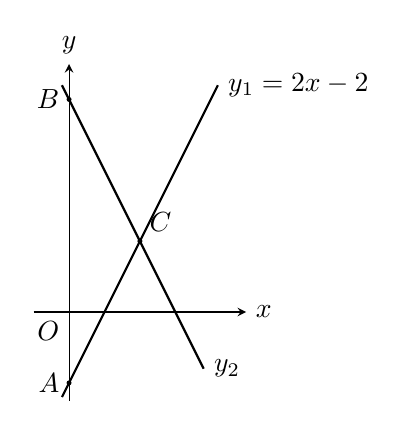
\begin{tikzpicture}[scale=0.45,>=stealth]
  \draw[->] (-1,0)--(5,0) node[right] {$x$};
  \draw[->] (0,-2.5)--(0,7) node[above] {$y$};
  \draw[thick] (-0.2,-2.4)--(4.2,6.4) node[right] {$y_1=2x-2$};
  \draw[thick] (-0.2,6.4)--(3.8,-1.6) node[right] {$y_2$};
  \fill (0,-2) circle (2pt) node[left] {$A$};
  \fill (0,6) circle (2pt) node[left] {$B$};
  \fill (2,2) circle (2pt) node[above right] {$C$};
  \node[below left] at (0,0) {$O$};
\end{tikzpicture}
}
\end{diagramcoltikz}
\end{eduProblemBlock}





\begin{eduAuxItem}{思路导航}
求已知直线上的交点 $C$$\;\to\;$用 $B,C$ 求 $y_2$$\;\to\;$用底高求面积$\;\to\;$分类讨论坐标轴上的 $P$\end{eduAuxItem}




\begin{eduSubQuestionItem}{例题 1}
完成本题的关键求解过程。\end{eduSubQuestionItem}

\begin{eduDualExplain}
  \begin{eduExplainLeft}
    \eduColumnTitle{\eduIconBulb}{小贴士}
        \eduSideHint{提示 1}{先用横坐标求 $C$，不要先设未知直线。}
        \eduSideHint{提示 2}{坐标轴上的点不是一种情况，$x$ 轴和 $y$ 轴要分开。}
  \end{eduExplainLeft}

  \begin{eduExplainRight}
    \eduColumnTitle{\eduIconBook}{解答}
      \eduExplainStep{1}{求已知直线上的交点 $C$}{由 $x_C=2$，代入 $y_1=2x-2$，得 $C(2,2)$。}
      \eduExplainStep{2}{用 $B,C$ 求 $y_2$}{直线 $y_2$ 过 $B(0,6)$、$C(2,2)$，斜率为 $-2$，故 $y_2=-2x+6$。}
      \eduExplainStep{3}{用底高求面积}{$AB=8$，点 $C$ 到 $y$ 轴距离为 $2$，所以 $S_{\triangle ABC}=\dfrac12\times8\times2=8$。}
      \eduExplainStep{4}{分类讨论坐标轴上的 $P$}{分别令 $P=(p,0)$ 与 $P=(0,p)$，按题目面积关系列方程，解得四个候选点。}
    \vspace{1mm}
    {\color{edu-blue}\bfseries\small 答案}\par\vspace{1mm}
    \begin{eduBulletList}
      \item (1) $C(2,2)$，$y_2=-2x+6$；(2) $8$；(3) $(-7,0),(9,0),(0,14),(0,-18)$。    \end{eduBulletList}
  \end{eduExplainRight}
\end{eduDualExplain}




\begin{eduMistakeBox}
\eduSubTitle{易错提醒}坐标轴上的点不是一种情况，$x$ 轴和 $y$ 轴要分开。\end{eduMistakeBox}




\begin{eduSummaryBlock}{\eduIconPin}{方法提醒}
\begin{eduBulletList}
  \item 先求交点，再求直线，再用面积条件分类找点。\end{eduBulletList}
\end{eduSummaryBlock}



\clearpage
\eduSectionTitle{例题二：输液剩余量图像与实际流速}


\begin{eduSolutionBox}{核心结论：输液剩余量图像与实际流速}
  \begingroup
  \setlength{\parskip}{2.5mm}
剩余量 $y$ 随时间 $x$ 线性下降，斜率的绝对值就是每分钟实际流速。\par
毫升/分钟与毫升/小时换算时要乘或除以 $60$。\par
  \endgroup
\end{eduSolutionBox}




\begin{eduProblemBlock}[例题 2]
\noindent
\begin{minipage}[t]{\dimexpr\linewidth-60mm-6mm\relax}
\vspace{0pt}
为提高控制输液从而减少因差异导致的药效不良事件，医疗输液器中的滴壶调节器从滚轮式改进为掣扣式的控制式。小明发现，在相同挡位下，不同粘度的液体流速存在差异，于是展开实验研究。（实验假设：对于掣扣式输液器设定的任意一个挡位，同样液体的输液速度保持恒定。）
\begin{enumerate}[label=(\arabic*)]
  \item 小明用掣扣式输液器设定每小时 $120$ 毫升的档位测试液体 $A$ 的流速，输液段内初始药液量为 $250$ 毫升，得到输液段剩余药液量 $y$（毫升）和时间 $x$（分钟）之间的关系如图所示。求 $y$ 关于 $x$ 的函数解析式（不写定义域）。
  \item 判断液体 $A$ 的实际流速是否与设定流速（$120$ 毫升/小时）一致；若不一致，假设实际流速与设定流速成正比，求要达到每小时 $120$ 毫升的流速应设定为多少毫升/小时。
  \item 用相同档位测试液体 $B$ 和液体 $C$ 的实际流速，发现液体 $B$ 的流速比液体 $C$ 每小时快 $60$ 毫升，且输完 $250$ 毫升液体 $C$ 所需时间是输完 $200$ 毫升液体 $B$ 所需时间的 $2$ 倍，求该档位下液体 $B$ 和液体 $C$ 的实际流速。
\end{enumerate}
\end{minipage}\hfill
\begin{diagramcoltikz}{60mm}{剩余药液量随时间变化}
\begin{tikzpicture}[scale=0.045,>=stealth]
  \draw[->] (0,0)--(52,0) node[right] {$x$（分钟）};
  \draw[->] (0,180)--(0,260) node[above] {$y$（毫升）};
  \draw[thick] (0,250)--(45,182.5);
  \draw[dashed] (20,180)--(20,220)--(0,220);
  \node[below] at (20,180) {$20$}; \node[left] at (0,220) {$220$}; \node[left] at (0,250) {$250$};
\end{tikzpicture}
}
\end{diagramcoltikz}
\end{eduProblemBlock}





\begin{eduAuxItem}{思路导航}
由图像求液体 A 的函数式$\;\to\;$换算实际流速$\;\to\;$按比例反推设定值$\;\to\;$列方程求 B、C 流速\end{eduAuxItem}




\begin{eduSubQuestionItem}{例题 2}
完成本题的关键求解过程。\end{eduSubQuestionItem}

\begin{eduDualExplain}
  \begin{eduExplainLeft}
    \eduColumnTitle{\eduIconBulb}{小贴士}
        \eduSideHint{提示 1}{图像纵轴是“剩余量”，不是“已经输完的量”。}
        \eduSideHint{提示 2}{小时和分钟混在一起时，先统一单位。}
  \end{eduExplainLeft}

  \begin{eduExplainRight}
    \eduColumnTitle{\eduIconBook}{解答}
      \eduExplainStep{1}{由图像求液体 A 的函数式}{图像过 $(0,250)$ 与 $(20,220)$，斜率为 $-\dfrac32$，故 $y=-\dfrac32x+250$。}
      \eduExplainStep{2}{换算实际流速}{每分钟减少 $1.5$ 毫升，实际流速为 $1.5\times60=90$ 毫升/小时。}
      \eduExplainStep{3}{按比例反推设定值}{实际/设定为 $90/120=3/4$，要实际达到 $120$，设定值应为 $120\div\dfrac34=160$。}
      \eduExplainStep{4}{列方程求 B、C 流速}{设液体 C 流速为 $v$，液体 B 为 $v+60$，由 $250/v=2\cdot200/(v+60)$ 解得 $v=100$。}
    \vspace{1mm}
    {\color{edu-blue}\bfseries\small 答案}\par\vspace{1mm}
    \begin{eduBulletList}
      \item (1) $y=-\dfrac32x+250$；液体 A 实际流速 $90$ 毫升/小时，不一致；应设定为 $160$ 毫升/小时。(2) 液体 B 为 $160$ 毫升/小时，液体 C 为 $100$ 毫升/小时。    \end{eduBulletList}
  \end{eduExplainRight}
\end{eduDualExplain}




\begin{eduMistakeBox}
\eduSubTitle{易错提醒}小时和分钟混在一起时，先统一单位。\end{eduMistakeBox}




\begin{eduSummaryBlock}{\eduIconPin}{方法提醒}
\begin{eduBulletList}
  \item 实际问题先读斜率含义，再做单位换算和比例方程。\end{eduBulletList}
\end{eduSummaryBlock}



\clearpage
\eduSectionTitle{例题三：交通流量一次函数与分段决策}


\begin{eduSolutionBox}{核心结论：交通流量一次函数与分段决策}
  \begingroup
  \setlength{\parskip}{2.5mm}
表格中等间隔数据可用两点求一次函数。\par
决策条件要先判断哪个方向流量更大，再与总量比例比较。\par
  \endgroup
\end{eduSolutionBox}




\begin{eduProblemBlock}[例题 3]
\noindent
\begin{minipage}[t]{\dimexpr\linewidth-60mm-6mm\relax}
\vspace{0pt}
某条东西方向道路双向共有三条车道，在早晚高峰经常会拥堵。数学研究小组希望改善道路拥堵情况，他们对该路段的交通量（辆/分钟）和时间进行统计分析，得到表格，并发现时间和交通量的变化规律符合一次函数的特征。
\begin{enumerate}[label=(\arabic*)]
  \item 请用一次函数分别表示 $y_1$ 与 $x$、$y_2$ 与 $x$ 之间的函数关系（不写定义域）。
  \item 如图，同学们希望设置可变车道来改善拥堵情况，根据车流量情况改变可变车道的行车方向。单位时间内东西向交通总量为 $y_0=y_1+y_2$，车流量大的方向交通量为 $v_m$；当 $v_m\ge\dfrac23y_0$，需使可变车道行车方向与拥挤方向相同。该路段从 $8$ 时至 $20$ 时，何时设置可变车道行车方向以缓解交通拥堵，并说明理由。
\end{enumerate}
\end{minipage}\hfill
\begin{diagramcoltikz}{60mm}{可变车道示意}
\begin{tikzpicture}[scale=0.65,>=stealth]
  \draw[thick] (0,0)--(6,0); \draw[thick] (0,1.2)--(6,1.2);
  \draw[dashed] (0,0.4)--(6,0.4); \draw[dashed] (0,0.8)--(6,0.8);
  \draw[->,thick] (1,0.2)--(4.8,0.2) node[right] {东};
  \draw[<-,thick] (1,1.0)--(4.8,1.0) node[left] {西};
  \node at (3,0.6) {可变车道};
\end{tikzpicture}
}
\end{diagramcoltikz}
\end{eduProblemBlock}





\begin{eduAuxItem}{思路导航}
由表格写出两个函数$\;\to\;$写出总量与阈值$\;\to\;$自东向西占优时判断$\;\to\;$自西向东占优时判断\end{eduAuxItem}




\begin{eduSubQuestionItem}{例题 3}
完成本题的关键求解过程。\end{eduSubQuestionItem}

\begin{eduDualExplain}
  \begin{eduExplainLeft}
    \eduColumnTitle{\eduIconBulb}{小贴士}
        \eduSideHint{提示 1}{不要只比较 $y_1,y_2$，还要满足“至少占总量三分之二”。}
        \eduSideHint{提示 2}{方向判断和比例判断是两步，不要合成一步。}
  \end{eduExplainLeft}

  \begin{eduExplainRight}
    \eduColumnTitle{\eduIconBook}{解答}
      \eduExplainStep{1}{由表格写出两个函数}{$y_1$ 每 3 小时增加 6，斜率为 $2$，故 $y_1=2x-6$；$y_2$ 每 3 小时减少 3，故 $y_2=-x+33$。}
      \eduExplainStep{2}{写出总量与阈值}{$y_0=y_1+y_2=x+27$，阈值为 $\dfrac23y_0=\dfrac23(x+27)$。}
      \eduExplainStep{3}{自东向西占优时判断}{当 $8\le x\le13$，$y_2\ge y_1$。解 $y_2\ge\dfrac23y_0$，得 $x\le9$。}
      \eduExplainStep{4}{自西向东占优时判断}{当 $13\le x\le20$，$y_1\ge y_2$。解 $y_1\ge\dfrac23y_0$，得 $x\ge18$。}
    \vspace{1mm}
    {\color{edu-blue}\bfseries\small 答案}\par\vspace{1mm}
    \begin{eduBulletList}
      \item $y_1=2x-6$，$y_2=-x+33$；$8\le x\le9$ 时设置为自东向西，$18\le x\le20$ 时设置为自西向东。    \end{eduBulletList}
  \end{eduExplainRight}
\end{eduDualExplain}




\begin{eduMistakeBox}
\eduSubTitle{易错提醒}方向判断和比例判断是两步，不要合成一步。\end{eduMistakeBox}




\begin{eduSummaryBlock}{\eduIconPin}{方法提醒}
\begin{eduBulletList}
  \item 表格建模后，先分方向，再用比例不等式筛选时间段。\end{eduBulletList}
\end{eduSummaryBlock}



\clearpage
\eduSectionTitle{例题四：分移函数与矩形交点分类}


\begin{eduSolutionBox}{核心结论：分移函数与矩形交点分类}
  \begingroup
  \setlength{\parskip}{2.5mm}
分段函数先看 $x\ge0$ 还是 $x<0$，再代入对应表达式。\par
与矩形恰好有几个交点，本质是直线段穿过矩形边界的分类。\par
  \endgroup
\end{eduSolutionBox}




\begin{eduProblemBlock}[例题 4]
\noindent
\begin{minipage}[t]{\dimexpr\linewidth-60mm-6mm\relax}
\vspace{0pt}
定义：形如 $y=\begin{cases}kx+b,&x\ge0,\\kx-b,&x<0\end{cases}$ 的函数称为正比例函数 $y=kx\ (k\ne0)$ 的“分移函数”，其中 $b$ 叫“分移值”。
\begin{enumerate}[label=(\arabic*)]
  \item 函数 $y=x$ 的“分移函数”为 $y=\begin{cases}x+3,&x\ge0,\\x-3,&x<0\end{cases}$，其中“分移值”为 $3$，在图中画出其图象；已知点 $(1,2k)$ 在 $y=kx\ (k\ne0)$ 的“分移函数” $y=\begin{cases}kx+6,&x\ge0,\\kx-6,&x<0\end{cases}$ 的图象上，求 $k$。
  \item 已知点 $P_1(2,1-m)$、$P_2(-3,2m+1)$ 在函数 $y=2x$ 的“分移函数”的图象上，求 $m$ 的值。
  \item 已知矩形 $ABCD$ 顶点坐标为 $A(1,0)$，$B(1,2)$，$C(-2,2)$，$D(-2,0)$，函数 $y=kx$ 的“分移函数”的“分移值”为 $3$，且其图象与矩形 $ABCD$ 恰好有 $2$ 个交点，请直接写出 $k$ 的取值范围。
\end{enumerate}
\end{minipage}\hfill
\begin{diagramcoltikz}{60mm}{分移函数与矩形窗口}
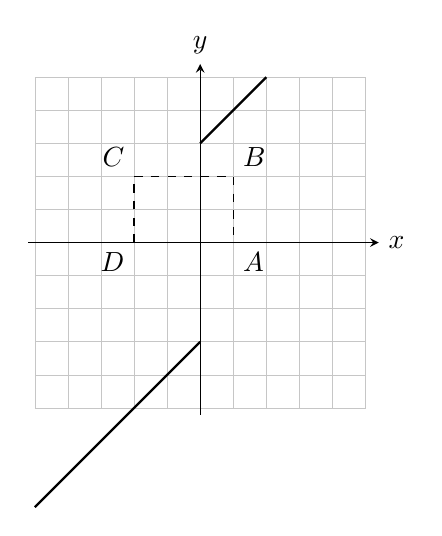
\begin{tikzpicture}[scale=0.42,>=stealth]
  \draw[step=1,gray!45,very thin] (-5,-5) grid (5,5);
  \draw[->] (-5.2,0)--(5.4,0) node[right] {$x$};
  \draw[->] (0,-5.2)--(0,5.4) node[above] {$y$};
  \draw[thick] (-5,-8)--(0,-3);
  \draw[thick] (0,3)--(2,5);
  \draw[dashed] (-2,0)--(-2,2)--(1,2)--(1,0);
  \node[above right] at (1,2) {$B$}; \node[above left] at (-2,2) {$C$};
  \node[below left] at (-2,0) {$D$}; \node[below right] at (1,0) {$A$};
\end{tikzpicture}
}
\end{diagramcoltikz}
\end{eduProblemBlock}





\begin{eduAuxItem}{思路导航}
按 $x$ 的符号代点$\;\to\;$用两点反求分移值$\;\to\;$分别看左右两段与矩形$\;\to\;$合并恰好两个交点的范围\end{eduAuxItem}




\begin{eduSubQuestionItem}{例题 4}
完成本题的关键求解过程。\end{eduSubQuestionItem}

\begin{eduDualExplain}
  \begin{eduExplainLeft}
    \eduColumnTitle{\eduIconBulb}{小贴士}
        \eduSideHint{提示 1}{新定义题不要急着套公式，先把定义拆成两段。}
        \eduSideHint{提示 2}{“恰好 2 个交点”要数边界交点，端点重合也只算一个点。}
  \end{eduExplainLeft}

  \begin{eduExplainRight}
    \eduColumnTitle{\eduIconBook}{解答}
      \eduExplainStep{1}{按 $x$ 的符号代点}{点 $(1,2k)$ 落在 $x\ge0$ 分支，代入 $2k=k+6$，得 $k=6$。}
      \eduExplainStep{2}{用两点反求分移值}{对 $y=2x$ 的分移函数设分移值为 $b$，由 $P_1,P_2$ 分别代入两段，解得 $m=-4$。}
      \eduExplainStep{3}{分别看左右两段与矩形}{右段 $y=kx+3$ 在 $0\le x\le1$，左段 $y=kx-3$ 在 $-2\le x<0$，分别判断是否穿过矩形 $0\le y\le2$。}
      \eduExplainStep{4}{合并恰好两个交点的范围}{计数后只有右段穿过矩形、左段不穿过时恰好两个交点，得 $-\dfrac32<k<-1$。}
    \vspace{1mm}
    {\color{edu-blue}\bfseries\small 答案}\par\vspace{1mm}
    \begin{eduBulletList}
      \item (1) $k=6$；(2) $m=-4$；(3) $-\dfrac32<k<-1$。    \end{eduBulletList}
  \end{eduExplainRight}
\end{eduDualExplain}




\begin{eduMistakeBox}
\eduSubTitle{易错提醒}“恰好 2 个交点”要数边界交点，端点重合也只算一个点。\end{eduMistakeBox}




\begin{eduSummaryBlock}{\eduIconPin}{方法提醒}
\begin{eduBulletList}
  \item 分段函数题先分段代入，再按图形边界做交点个数分类。\end{eduBulletList}
\end{eduSummaryBlock}




\end{document}
